\chapter{Código fonte de um Universo Conceitual como nuvem de palavras sobre o improviso de códigos}\label{app:A}

Apresentamos no exemplo A.1 o código-fonte, em linguagem python, utilizado para extração parcial do espaço conceitual da pesquisa (\autoref{fig:nuvemlivecoding}, p.~\pageref{fig:nuvemlivecoding}). A biblioteca utilizada, \emph{Wordcloud}, pode ser encontrada em \url{https://github.com/amueller/word_cloud}.

O Código abaixo considera a seguinte situação: é possível converter um arquivo de texto em formato \emph{.pdf} para formato \emph{.txt}. Feita a conversão, é possível realizar um levantamento estatístico das palavras mais usadas (o que pode, parcialmente, indicar idéias e conceitos).

 Existem programas online, como o encontrado no link \url{http://convertonlinefree.com/PDFToTXTEN.aspx}, que realizam a conversão. É necessária a correção de alguns erros de caracteres (ver \autoref{fig:utf8}). Além disso, informações de cabeçalho, códigos-fontes, e outros elementos de editoração, foram descartados por considerarmos que não eram parte do corpo textual. Em outras palavras, descartamos palavras que não faziam parte de um discurso de texto, ou atrapalhavam o processo de criação da imagem. O que por sí não resolve todos os problemas, mas auxilia na elaboração da imagem.

\begin{figure}[!h]
  \centering
  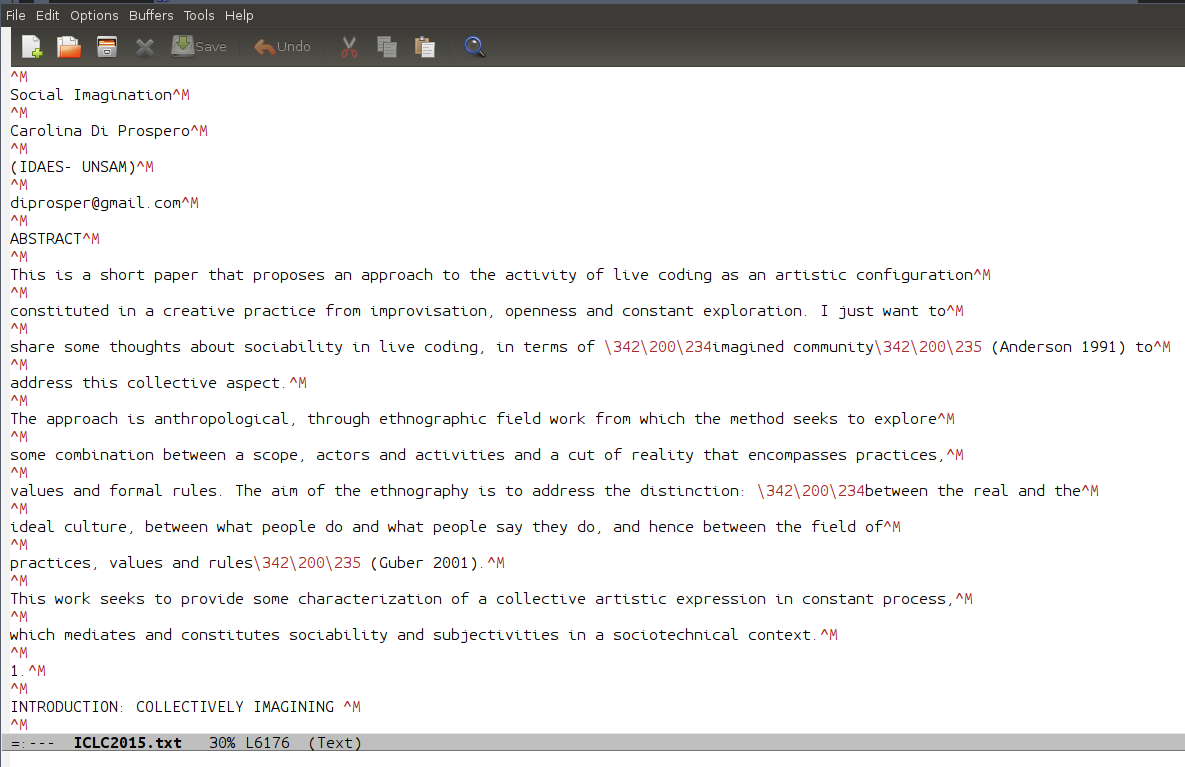
\includegraphics[scale=0.3]{imagens/utf8.png}
  \caption{Resultado da conversão do arquivo \emph{pdf} para \emph{txt} resulta em problemas de codificação que necessitaram ser corrigidos por comparação com o arquivo original. \textbf{Fonte}: autor.}
  \label{fig:utf8}
\end{figure}


\begin{example}{Código-fonte que utiliza a biblioteca wordcloud}  
\begin{minted}{python}
# Bibliotecas utilizadas
from urllib2 import urlopen
from bs4 import *
import re
import datetime
from iso import *
import matplotlib.pyplot as plt

from wordcloud import WordCloud
    
# Abra o arquivo em modo de leitura
# ICLC2015.txt: 
#   - um arquivo em modo de texto 
#     convertido de um conjunto de artigos
#   - Universo conceitual publicado
#     em 2015 na Inglaterra  
t = open("ICLC2015.txt", "r").read()

# Gere uma nuvem de palavras
wc = WordCloud().generate(t)
    
# Mostre a imagem gerada com o matplotlib,
# biblioteca para plotar imagens por dados numericos,
# levando em conta as frequencias das palavras
plt.figure()
plt.imshow(wc)
plt.axis("off")
plt.show()
\end{minted}
\label{cod:nuvem}
\end{example}

\section{Classes qualitativas de um Universo de conceitos do \emph{live coding}}

Com auxílio da biblioteca NLTK\footnote{Disponível em \url{http://nltk.org/}.}, categorizamos a nuvem de conceitos de acordo com sua função textual (ver exemplo B.1). 

\begin{example}{Categorização dos dados}
\begin{minted}{python}
# Importe bibliotecas
from os import path
from wordcloud import WordCloud
import math
import nltk

# Abra o arquivo em modo de leitura
t = open("assets/ICLC2015.txt", "r").read()
wc = WordCloud().generate(t)

# Organize as palavras por frequencia
# de presenca no texto
groups = [[] for i in range(10)]

for i, t in enumerate(wc.words_):
    freq = t[1]
    word = t[0]
    index = int(math.floor(freq*10))
    if freq >= index/10.0 and freq < (index+1)/10.0:
        print word
        print index
        groups[index-1].append(word)

# CLASSIFIQUE AS PALAVRAS
groups = [nltk.pos_tag(e) for e in groups]
print groups
\end{minted}
\label{cod:classes}
\end{example}

O código acima gerou uma saída textual que foi reorganizada na tabela \autoref{tab:comparacao}.

\begin{table}
\caption{Tabela de classes qualitativas de termos utilizados nos anais do ICLC2015, agrupados por funções textuais.}
\small
    \begin{tabular}{ | p{1.45cm} | p{1.3cm} | p{2cm} | p{1.45cm} | p{1.45cm} | p{1.45cm} | p{1.45cm} | p{1.45cm} | p{1.25cm} |}
    \hline 
    \hline 

    \tiny \textbf{Número Qualitativo/Função} & \textbf{0} & \textbf{1}  & \textbf{2} & \textbf{3} & \textbf{4}  & \textbf{5} & \textbf{8} & \textbf{9}\\
    \hline 
    \hline 

    \tiny \textbf{Pessoas}  
    & - 
    & \tiny Collins, Blackwell, McLean, Grossi 
    & - 
    & - 
    & - 
    & -  
    & - 
    & - \\
    \hline

    \tiny \textbf{Aplicativos}
    & - 
    & \tiny SuperCollider, Gibber, SonicPi  
    & - 
    & - 
    & - 
    & -  
    & - 
    & \\
    \hline
    
    \tiny \textbf{Verbos}  
    & \tiny take, see, shared, networked, explore, made
    & \tiny make, provide, writing, solving, making
    & \tiny used
    & \tiny using, coding  
    & \tiny performer
    & - 
    & - 
    & -  \\
  \hline

     \tiny \textbf{Adjetivo ou numeral, ordinal}  
    & \tiny less, open, potential, similar, important, cognitive, virtual
    & \tiny first, real, electronic, visual, ensemble, possible, free, livecoding, aspect  
    & \tiny musical, many
    & \tiny new, one
    & - 
    & -  
    & \tiny live 
    & - \\
    \hline

    \tiny \textbf{Substantivo}  
    & \tiny Browser, point, approach, order, node, collaborative, number, source, present, community, server, framework, orchestra, digital, level, kind, type, memory, analysis, line, body, concept, technology, working, org, current, show, mean, end, processes, people, international
    & \tiny University, conference, proceedings, network, interface, environment, text, form, context, musician, space, paper, program, audience, function, change, control, human, laptop, interaction, structure, part, session, tool, result, create, object, case, algorithm, value, development, material, set, technique, parameter, idea, screen, video, application, support, composition, piece, knowledge, feature, cell, activity, art, action, information, method, web, rule, group, need, particular, project, allow, collaboration, programmer, member, play, output 
    & \tiny use, coder, process, state, example, way, software, research, problem, experience, design, improvisation, different, machine, pattern, audio
    & \tiny work, instrument
    & \tiny system, computer, user, language, time, practice, sound
    & \tiny programming
    & \tiny performance, code
    & \tiny ``live coding'', music  \\
    \hline
    \hline
   
    \end{tabular}
\label{tab:comparacao}
\end{table}

Uma breve análise da nuvem de palavras \ver{fig:nuvemlivecoding},  pode elucidar parte das questões-satélites do \emph{live coding}. Na \autoref{tab:comparacao} filtrei parte dos resultados por conjuntos de funções textuais -- sujeitos-humanos, sujeitos-ferramentas, verbos, adjetivos e substantivos -- e quantas vezes foram utilizados, em categorias qualitativas (0, menos usado e 9 o mais usado, sendo que 6 e 7 não apresentaram resultados).

No caso dos sujeitos-humanos, podemos ver nomes de Nick Collins e Alex McLean, praticantes responsáveis pela criação de um manifesto, em parceria com \citeonline{ward_live_2004}. Pietro Grossi, é um personagem recentemente estudado por \citeonline{mori_pietro_2015} como um caso prematuro de \emph{live coding}, a partir do final da década de sessenta.

No caso dos sujeitos-ferramentas, destacamos o papel do \emph{SuperCollider}, já citado anteiormente, e do \emph{Gibber}\cite{roberts_gibber:_2012,wyse_viability_2014}\footnote{Disponível em \url{http://gibber.mat.ucsb.edu}}. Ambos são ambientes de programação para de síntese sonora e composição algorítmica. Uma característica em comum destes ambientes, o procedimento de compilação de códigos, é conhecido como \emph{Just In Time} \cite{aycock_brief_2003}, dispositivo técnico que permitiu a execução de códigos durante o tempo de execução.

Verbos fornecem informação sobre o comportamento dos improvisadores de códigos. Além da atividades como \emph{performatizar} e \emph{codificar}, é notável atividades sociais ligadas à visão, à escrita, à técnica, à lógica. Embora a Música seja a atividade proeminente do \emph{live coding}, não obtivemos resultados que retornassem, por exemplo, a palavra \emph{hearing}. 

Adjetivos destacam características da prática. \emph{Live} é a palavra-chave, e sugere uma prática de performance. \emph{Visual} sugere uma característica fundamental, tanto quanto a Música, para uma performance. \emph{Ensemble} destaca a natureza de grupos, isto é, poucas performances \emph{solo} são realizadas se comparadas às performances de \emph{duos}, \emph{trios}. 

Palavras como \emph{university}, \emph{research} e \emph{technology}, e \emph{laptop} acusam não apenas uma prática artística, mas um Programa de Investigação Científica. A esfera de pesquisa acadêmica permitiu ramos de desenvolvimento com linguagens de programação, cognição, inteligência artificial, semiologia, performance musical (improvisação), e mais recentemente, antropologia, conferindo à produção de \emph{live coding} espécie de autenticidade acadêmica.